Chương này tập trung vào việc mô tả hệ thống điều khiển đèn giao thông thông minh sử dụng thuật toán học tăng cường sâu (\ac{drl}). Hệ thống sẽ được huấn luyện và đánh giá trong môi trường giả lập \ac{sumo}, với dữ liệu đầu vào có thể được thu thập từ thực tế thông qua các camera tích hợp thuật toán nhận diện vật thể \ac{yl}.

\section{Kiến trúc tổng thể hệ thống}
Để có cái nhìn toàn diện về hệ thống điều khiển đèn giao thông thông minh, trước tiên, chúng ta cần tìm hiểu kiến trúc tổng thể của nó. Hệ thống này được thiết kế theo mô hình phân tầng, cho phép khả năng mở rộng linh hoạt từ việc điều khiển một giao lộ đơn lẻ đến việc điều phối đồng bộ nhiều giao lộ cùng lúc.

\subsection{Kiến trúc tổng quan}

\begin{figure*}[!htp]
    \centering
    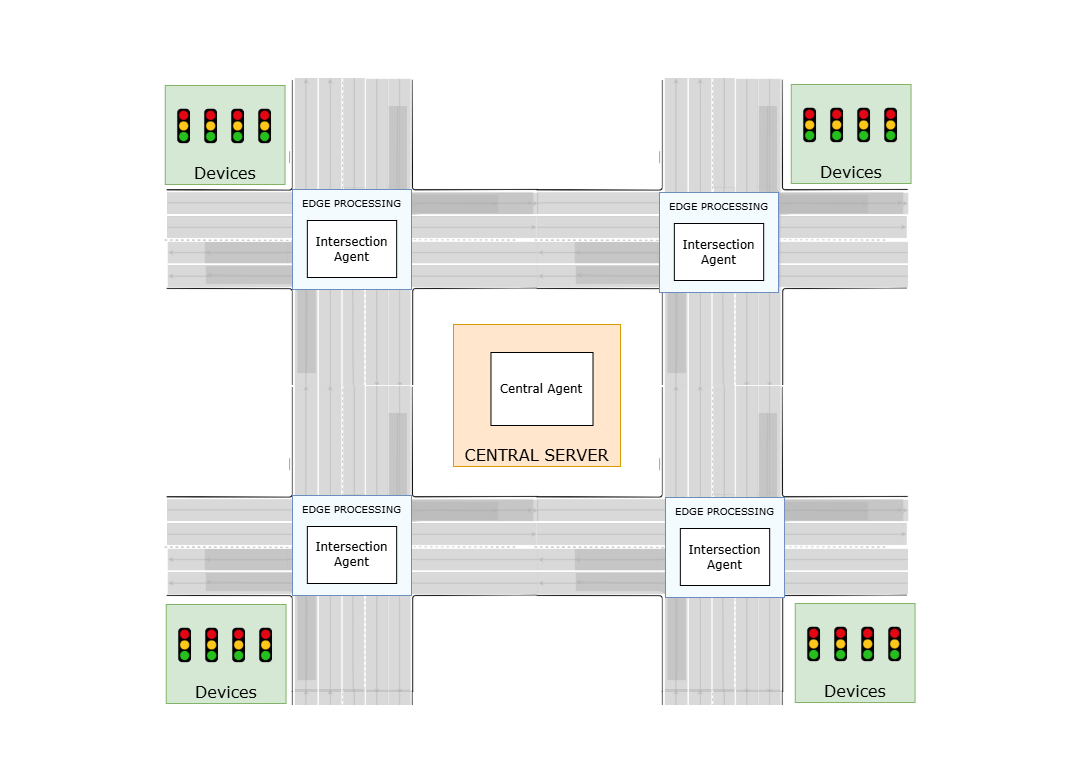
\includegraphics[width=\textwidth]{img/overview_architecture.png}
    \caption{Kiến trúc tổng quan hệ thống điều khiển đèn giao thông thông minh}
    \label{fig:overview_architecture}
\end{figure*}

Hình \ref{fig:overview_architecture} thể hiện kiến trúc tổng quan của hệ thống,
bao gồm các thành phần chính:

\begin{itemize}
    \item \textbf{Lớp thu thập dữ liệu:} Thu thập dữ liệu từ camera và sensors

    \item \textbf{Lớp xử lý:} Xử lý dữ liệu và nhận diện đối tượng

    \item \textbf{Lớp quyết định:} Các agent AI ra quyết định điều khiển

    \item \textbf{Lớp đồng bộ:} Đồng bộ hóa giữa các giao lộ

    \item \textbf{Lớp điều khiển:} Điều khiển đèn giao thông thực tế
\end{itemize}

\subsection{Kiến trúc chi tiết hệ thống}

\begin{figure*}[!htp]
    \centering
    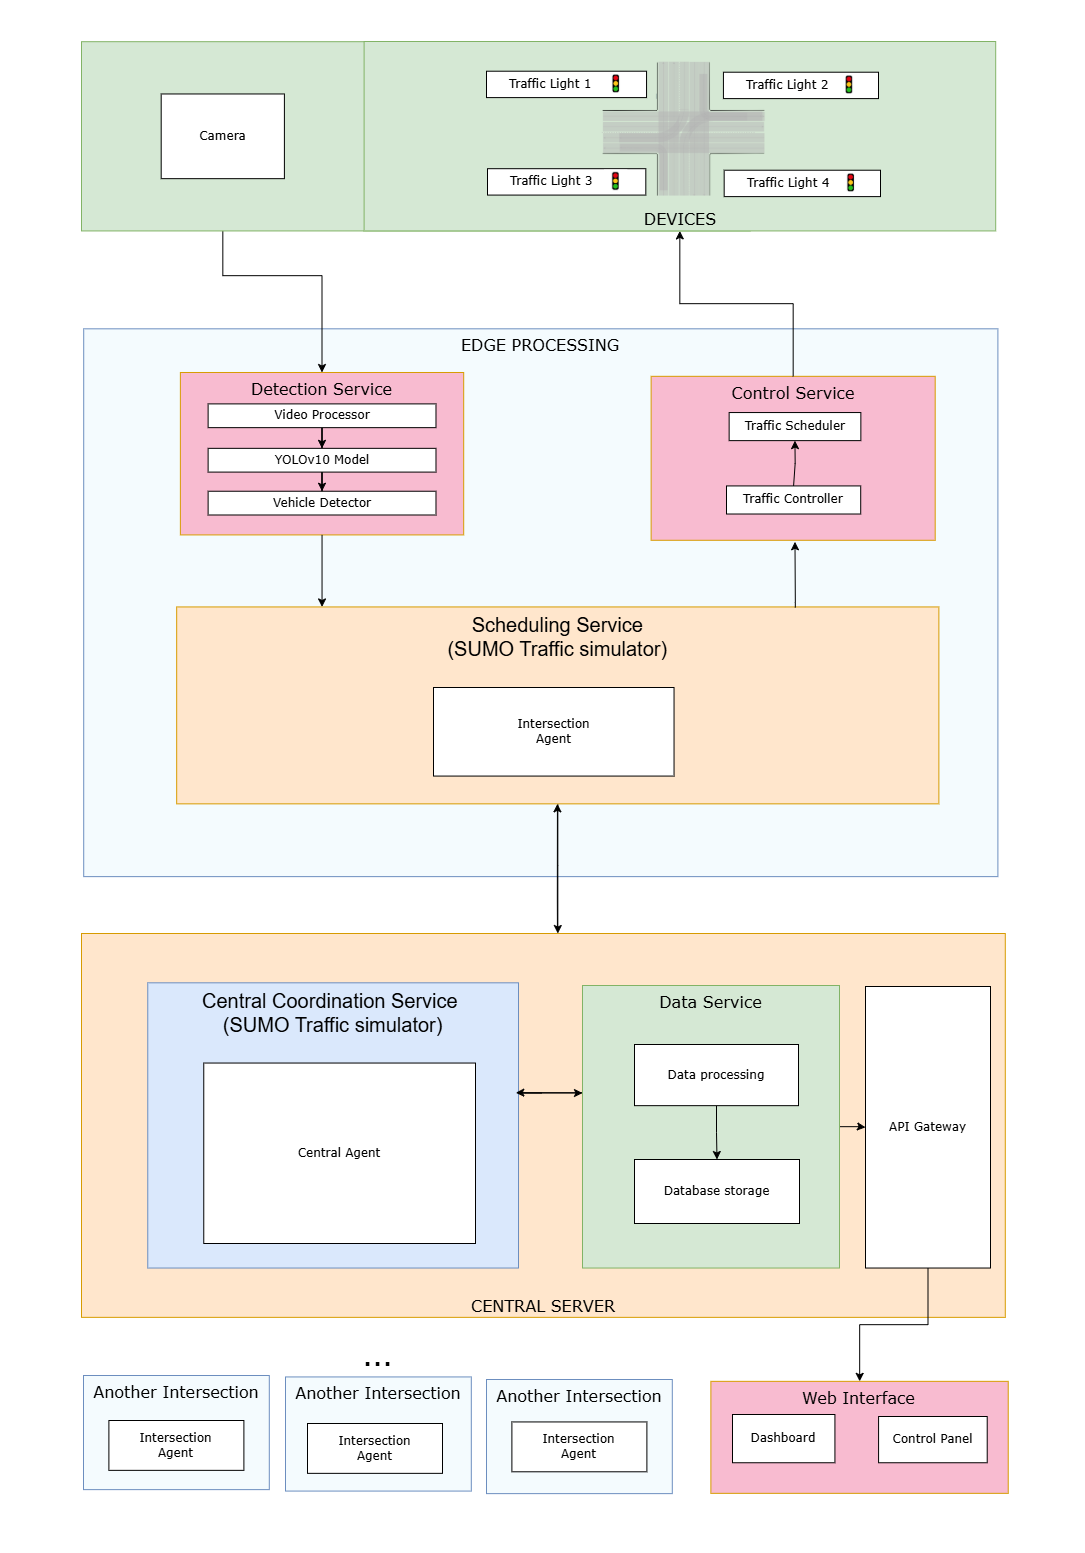
\includegraphics[width=0.7\textwidth]{img/detailed_architecture.png}
    \caption{Kiến trúc chi tiết hệ thống với các thành phần}
    \label{fig:detailed_architecture}
\end{figure*}

Mô tả chi tiết các thành phần và luồng dữ liệu trong hệ thống:

\begin{enumerate}
    \item \textbf{Lớp thiết bị:} Thu thập video từ các camera giám sát giao thông
    \item \textbf{Lớp xử lý biên}
    \begin{itemize}
        \item \textbf{Nhận diện phương tiện tham gia giao thông:} Dữ liệu video sẽ được dùng để nhận diện các phương tiện tham gia giao thông cũng như xác định khoảng cách và làn đường mà phương tiện đang di chuyển
        \item \textbf{Các tác nhân DQN :} Các tác nhân ngoài việc điều khiển đèn tín hiệu từng giao lộ thì còn có nhiệm vụ nhận các thông tin từ YOLO và giả lập tình trạng giao thông tại nút giao. Sau đó, gửi các thông tin cần thiết đến centtral server để dự doán và ra quyết định 
    \end{itemize}
    \item \textbf{Central Server:} Thu thập từ các tác nhân và chạy các mô hình DQN và Sync Agent để ra quyết định. Đồng thời, cung cấp giao diện để quan sát và điều khiển
\end{enumerate}

\section{Phương pháp mô phỏng dữ liệu từ camera}
\subsection{Mô hình nhận diện vật thể}
Để phát hiện và nhận diện phương tiện trong các luồng video giao thông, sử dụng mô hình \textbf{YOLO11}, phiên bản mới nhất trong chuỗi mô hình phát hiện đối tượng thời gian thực của \textbf{Ultralytics}. YOLO11 mang đến những cải tiến đáng kể về kiến trúc và phương pháp huấn luyện, giúp nâng cao độ chính xác, tốc độ và hiệu quả so với các phiên bản tiền nhiệm.

\begin{figure}[!htp]
    \centering
    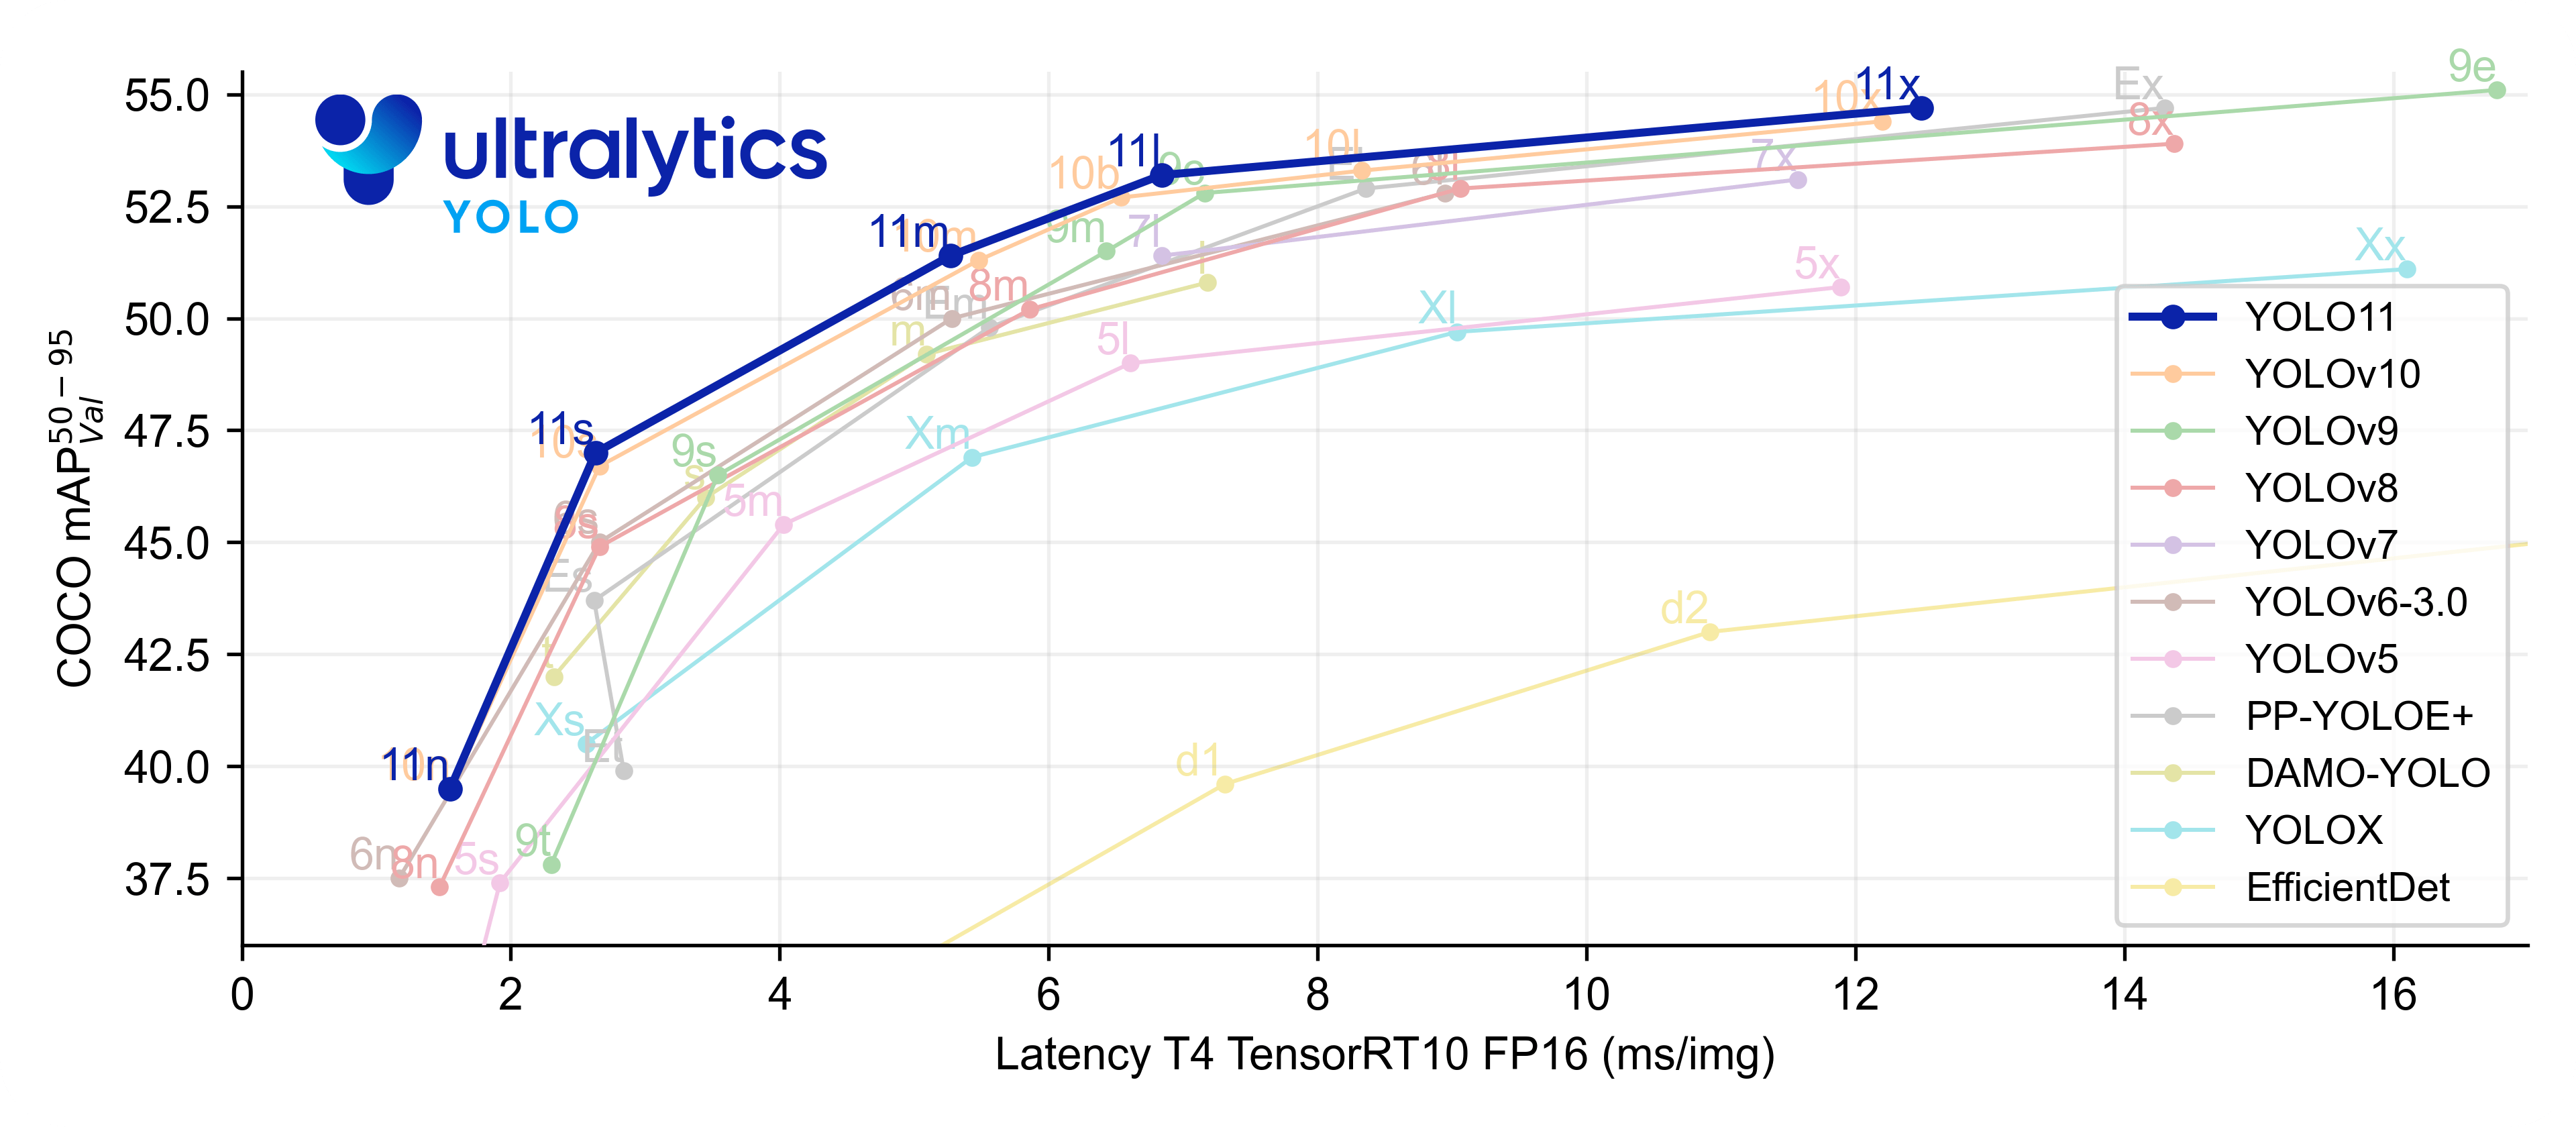
\includegraphics[width=\textwidth]{img/yolo_models}
    \caption{So sánh hiệu suất giữa các mô hình \footnotemark[1]}
    \label{fig:yolo_models}
\end{figure}
Cụ thể, nghiên cứu này sử dụng mô hình đã được huấn luyện trước (pre-trained) có tên là \textbf{\texttt{yolov11s.pt}}. Đây là phiên bản thu nhỏ của YOLO11, được lựa chọn dựa trên các ưu điểm nổi bật sau:

\begin{itemize}
    \item \textbf{Hiệu suất cân bằng:} Mô hình \texttt{yolov11s.pt} đạt được chỉ số mAP\textsuperscript{50-95} là 47.0 trên tập dữ liệu COCO, đồng thời có tốc độ xử lý rất nhanh (chỉ 2.5ms trên GPU Tesla T4). Sự cân bằng giữa độ chính xác cao và tốc độ suy luận nhanh là yếu tố then chốt cho các ứng dụng phân tích giao thông thời gian thực\footnote[1]{Ultralytics Documents: \url{https://docs.ultralytics.com/models/yolo11}}.
    \item \textbf{Kiến trúc hiệu quả:} YOLO11 được cải tiến về kiến trúc backbone và neck, giúp tăng cường khả năng trích xuất đặc trưng. Nhờ đó, các mô hình như YOLO11 đạt được độ chính xác cao hơn với số lượng tham số ít hơn, làm cho chúng hiệu quả hơn về mặt tính toán. Phiên bản \texttt{yolov11s.pt} chỉ có 9.4 triệu tham số.
    \item \textbf{Huấn luyện trên tập dữ liệu COCO:} Giống như các phiên bản trước, mô hình được huấn luyện sẵn trên tập dữ liệu COCO, bao gồm các lớp đối tượng giao thông quan trọng như \texttt{car}, \texttt{motorcycle}, \texttt{bus}, và \texttt{truck}. Điều này cho phép áp dụng mô hình trực tiếp vào bài toán mà không cần huấn luyện lại, giúp tiết kiệm thời gian và tài nguyên.
\end{itemize}
Với những lý do trên, mô hình \texttt{yolov11s.pt} được xác định là lựa chọn phù hợp nhất, đáp ứng được các yêu cầu về độ chính xác, tốc độ và hiệu quả cho hệ thống được đề xuất trong luận văn.

\subsection{Thuật toán theo dõi đối tượng}
\subsubsection{SORT}
SORT (Simple Online and Realtime Tracking) là một thuật toán theo dõi đối tượng đơn giản nhưng hiệu quả. Thuật toán này kết hợp giữa bộ lọc Kalman và thuật toán Hungarian để theo dõi các đối tượng qua nhiều khung hình video liên tiếp. Trong nghiên cứu này, SORT được sử dụng để theo dõi các phương tiện giao thông qua các khung hình video, giúp duy trì ID nhất quán cho mỗi phương tiện và thu thập thông tin về quỹ đạo di chuyển của chúng. SORT hoạt động theo các bước chính sau:

\begin{itemize}
    \item \textbf{Dự đoán vị trí:} Sử dụng bộ lọc Kalman để dự đoán vị trí của các đối tượng đã được theo dõi trong khung hình tiếp theo. Bộ lọc này mô hình hóa chuyển động của đối tượng dựa trên vận tốc và gia tốc.

    \item \textbf{Gán đối tượng:} Khi nhận được các phát hiện mới từ mô hình YOLO, SORT sử dụng thuật toán Hungarian để gán các phát hiện này với các đối tượng đang được theo dõi. Việc gán dựa trên khoảng cách IoU (Intersection over Union) giữa các hộp giới hạn dự đoán và phát hiện.

    \item \textbf{Cập nhật trạng thái:} Sau khi gán thành công, bộ lọc Kalman được cập nhật với thông tin mới từ các phát hiện. Các đối tượng không được gán trong một số khung hình liên tiếp sẽ bị loại bỏ khỏi danh sách theo dõi.
\end{itemize}

Ưu điểm chính của SORT là:
\begin{itemize}
    \item \textbf{Tốc độ xử lý cao:} Thuật toán có thể xử lý video với tốc độ khung hình cao, phù hợp cho các ứng dụng thời gian thực.

    \item \textbf{Độ chính xác tốt:} Đạt được độ chính xác cao trong việc theo dõi các đối tượng chuyển động với tốc độ vừa phải.

    \item \textbf{Tính đơn giản:} Dễ dàng triển khai và tích hợp với các mô hình phát hiện đối tượng khác nhau.
\end{itemize}

Tuy nhiên, SORT cũng có một số hạn chế:
\begin{itemize}
    \item \textbf{Không xử lý tốt các trường hợp che khuất:} Khi đối tượng bị che khuất hoàn toàn trong một khoảng thời gian, thuật toán có thể mất dấu đối tượng đó.

    \item \textbf{Không duy trì ID khi đối tượng tái xuất hiện:} Nếu một đối tượng biến mất và xuất hiện lại, nó sẽ được gán một ID mới.
\end{itemize}

\subsubsection{BotSORT}
BotSORT (Boosting SORT) là một phiên bản cải tiến của thuật toán SORT, được tích hợp trong thư viện Ultralytics. Đây là thuật toán chính được dùng trong nghiên cứu, thuật toán này khắc phục các hạn chế của SORT bằng cách bổ sung thêm các tính năng:

\begin{itemize}
    \item \textbf{Camera Motion Compensation (CMC):} BotSORT sử dụng kỹ thuật bù chuyển động camera để xử lý các trường hợp camera di chuyển hoặc rung lắc. Điều này giúp cải thiện độ chính xác trong việc theo dõi đối tượng khi góc nhìn thay đổi.

    \item \textbf{Appearance Feature Matching:} Khác với SORT chỉ dựa vào IoU, BotSORT kết hợp thêm việc so khớp đặc trưng hình ảnh (appearance features) để xác định đối tượng. Điều này giúp:
        \begin{itemize}
            \item Duy trì ID nhất quán ngay cả khi đối tượng bị che khuất tạm thời
            \item Giảm thiểu việc gán sai ID khi có nhiều đối tượng tương tự xuất hiện
            \item Cải thiện khả năng theo dõi trong các trường hợp phức tạp
        \end{itemize}

    \item \textbf{Improved State Estimation:} BotSORT sử dụng một phiên bản cải tiến của bộ lọc Kalman, cho phép:
        \begin{itemize}
            \item Dự đoán chính xác hơn về vị trí và vận tốc của đối tượng
            \item Xử lý tốt hơn các trường hợp chuyển động không đều
            \item Giảm thiểu việc mất dấu đối tượng khi có sự thay đổi đột ngột về hướng di chuyển
        \end{itemize}
\end{itemize}

Trong nghiên cứu này, BotSORT được sử dụng như một lựa chọn thay thế cho SORT trong các trường hợp cần độ chính xác cao hơn, đặc biệt là khi:
\begin{itemize}
    \item Có nhiều phương tiện di chuyển gần nhau và có thể che khuất lẫn nhau

    \item Camera có thể bị rung lắc hoặc di chuyển

    \item Cần duy trì ID nhất quán cho các phương tiện trong thời gian dài
\end{itemize}

\section{Thiết lập môi trường mô phỏng giao thông đô thị SUMO}

\begin{figure}[!htp]
    \centering
    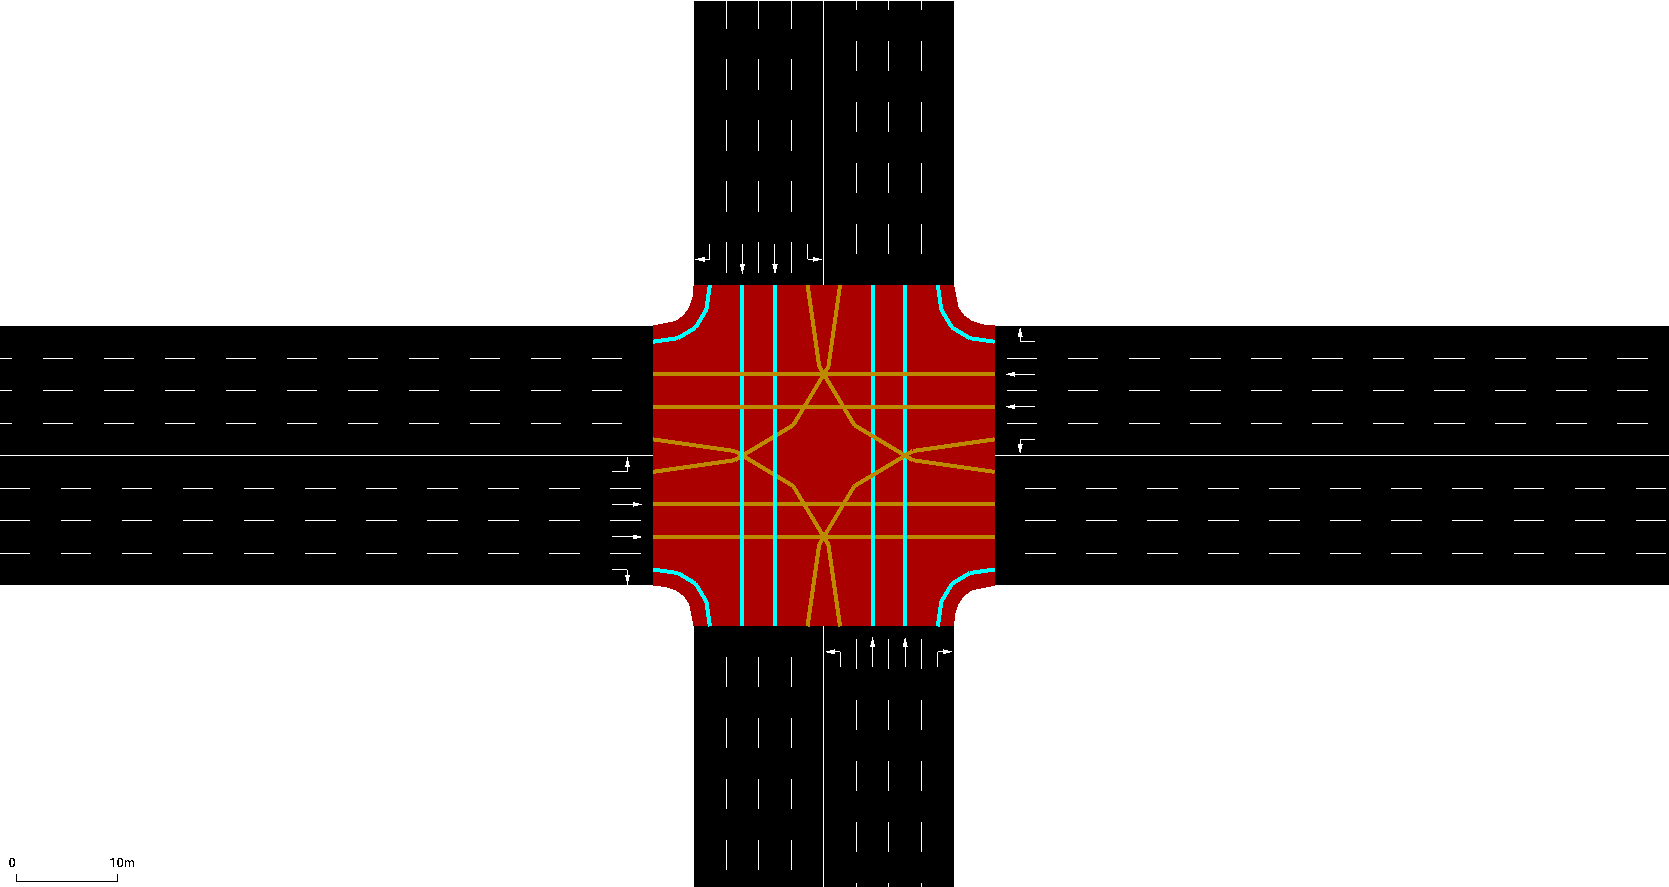
\includegraphics[width=\textwidth]{figures/sumo_map}
    \caption{Mô hình giao lộ trong mô phỏng}
    \label{fig:sumo_map}
\end{figure}

Nhóm nghiên cứu mô phỏng một nút giao thông trong SUMO với bốn làn đường, với thiết lập điều hướng cụ thể để kiểm soát hướng di chuyển của phương tiện. Cụ thể:
\begin{itemize}
    \item Làn trái ngoài: Chỉ được phép rẽ trái.

    \item 2 Làn giữa: Chỉ được phép đi thẳng.

    \item Làn trong cùng: Chỉ được phép rẽ phải.
\end{itemize}

\section{Xây dựng mô hình DRL}
\subsection{Định nghĩa môi trường (Environment)}
Trong khuôn khổ của đề tài, môi trường chính là một kịch bản giao thông được giả lập bởi \ac{sumo}. Một lớp (class) `Simulation` trong Python được tạo ra để quản lý và tương tác với môi trường này. Lớp `Simulation` đóng vai trò trung gian, thực
hiện các công việc sau:
\begin{itemize}
    \item Khởi tạo và kết thúc một phiên giả lập \ac{sumo} thông qua thư viện
        TraCI.

    \item Tại mỗi bước thời gian, thu thập dữ liệu thô từ \ac{sumo} để xây dựng \textit{trạng
        thái}.

    \item Gửi các \textit{hành động} (lựa chọn pha đèn) từ agent đến \ac{sumo} để
        thực thi.

    \item Tính toán \textit{phần thưởng} dựa trên kết quả của hành động vừa thực
        hiện.

    \item Quản lý vòng lặp của một tập (episode) huấn luyện, bao gồm việc tạo ra
        các luồng giao thông ngẫu nhiên cho mỗi tập.
\end{itemize}

\subsection{Định nghĩa tác nhân (Agent)}
Agent là một thực thể ra quyết định, trong trường hợp này là mô hình \ac{drl} được
xây dựng bằng thư viện TensorFlow và Keras. Agent này thực hiện hai nhiệm vụ
chính:
\begin{enumerate}
    \item \textbf{Dự đoán (Inference):} Dựa vào \textit{trạng thái} hiện tại của
        môi trường, agent sử dụng mạng neural của mình để dự đoán giá trị Q (Q-value)
        cho mỗi \textit{hành động} có thể thực hiện. Hành động có giá trị Q cao
        nhất sẽ được lựa chọn (chiến lược tham lam).

    \item \textbf{Học (Learning):} Agent sử dụng một bộ nhớ đệm gọi là \textit{Experience
        Replay} để lưu trữ các kinh nghiệm $(s, a, r, s')$. Trong giai đoạn huấn
        luyện, nó sẽ lấy ra các lô (batch) kinh nghiệm ngẫu nhiên từ bộ nhớ này để
        cập nhật trọng số của mạng neural, nhằm cải thiện khả năng dự đoán và ra
        quyết định trong tương lai.
\end{enumerate}
Quá trình lựa chọn hành động tuân theo chính sách $\epsilon$-greedy: với một xác
suất nhỏ $\epsilon$, agent sẽ chọn một hành động ngẫu nhiên (thăm dò), và trong
thời gian còn lại, nó sẽ chọn hành động tốt nhất dựa trên dự đoán của mô hình (khai
thác).

\subsection{Thiết kế trạng thái (State)}
Trạng thái là cách biểu diễn thông tin của môi trường để agent có thể hiểu và ra quyết định. Trong mô hình này, trạng thái được định nghĩa là một vector một chiều có 80 phần tử biểu diễn vị trí và mật độ xe tại các là đường tại mỗi bước. Sau đây là các bước ghi nhận thông tin vào trạng thái.

\begin{figure}[!htp]
    \centering
    \begin{subfigure}[b]{0.45\textwidth}
        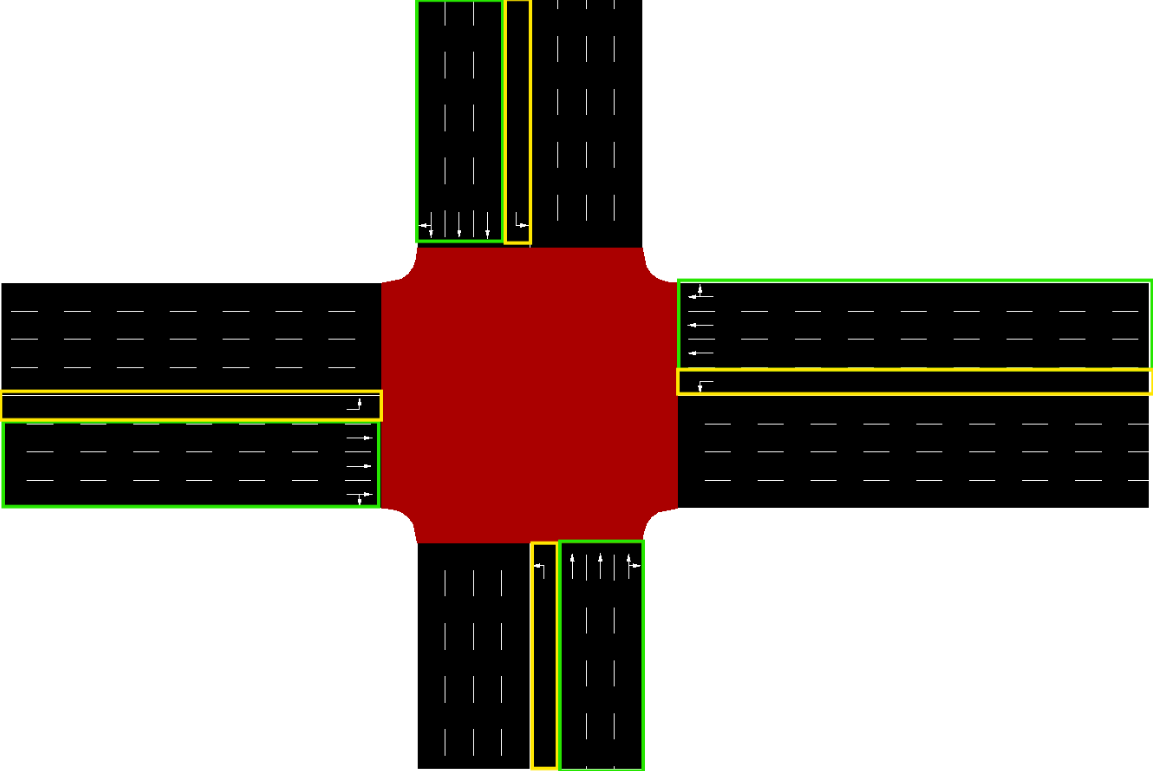
\includegraphics[width=\textwidth]{img/sumo_state_1.png}
        \caption{Hai nhóm làn đường}
        \label{fig:sumo_state_1}
    \end{subfigure}
    \hfill
    \begin{subfigure}[b]{0.45\textwidth}
        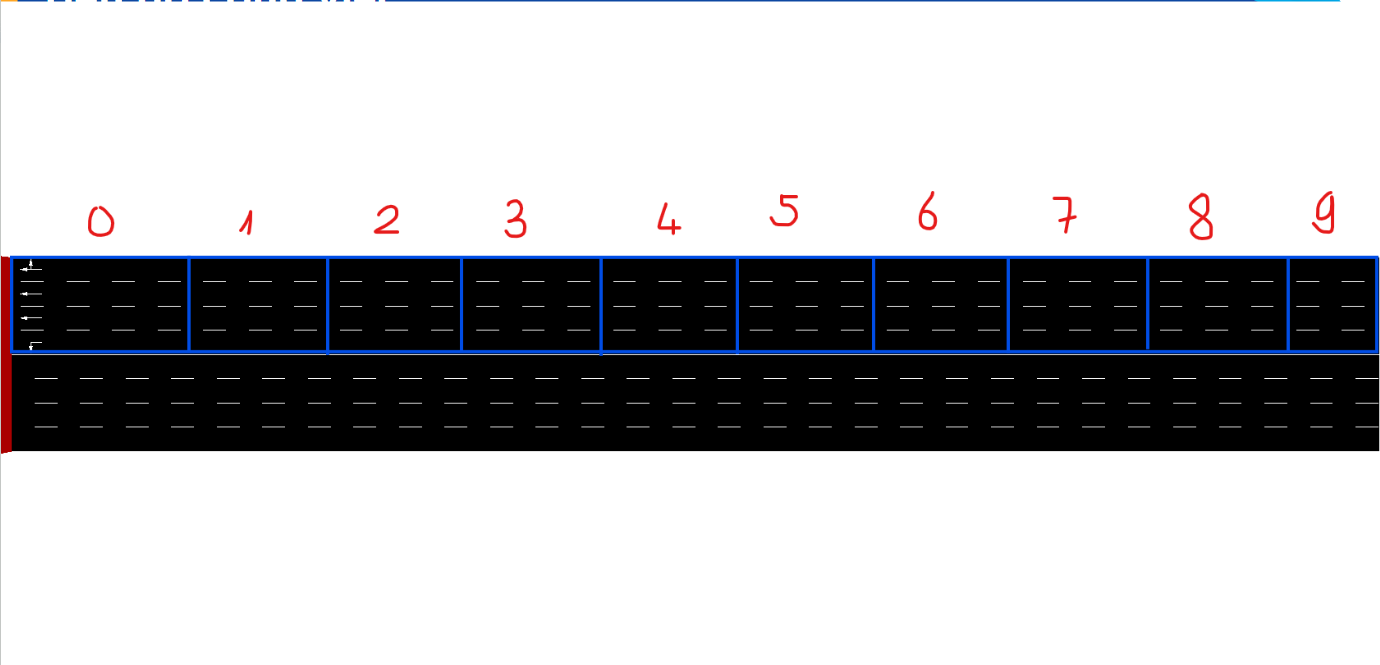
\includegraphics[width=\textwidth]{img/sumo_state_2.png}
        \caption{Chia làn đường thành 10 phần}
        \label{fig:sumo_state_2}
    \end{subfigure}
    \caption{Tiêu đề chung cho cả hai hình}
    \label{fig:sumo_state}
\end{figure}

\begin{enumerate}
    \item \textbf{Phân loại làn đường:} Chia con đường kết nối tới nút giao thành 2 nhóm làn đường như trong hình \ref{fig:sumo_state_1}: nhóm màu vàng bao gồm làn đường chỉ được rẻ trái và nhóm màu xanh bao gồm các làn đường được đi thẳng và rẻ phải. Với mỗi con đường có 2 nhóm làn đường thì tổng cộng có tất cả 8 nhóm làn đường. Các nhóm sẽ được đánh số theo chiều kim đồng hồ, nhóm làn màu xanh lá sẽ được đánh số chẵn và nhóm làn đường màu vàng sẽ được đánh số lẻ.
    \item \textbf{Chia các làn đường theo từng ô:} Mỗi làn đường có chiều dài bằng tầm quan sát được của camera giám sát và được chia thành 10 phần như hình \ref{fig:sumo_state_2}. Trạng thái sẽ ghi nhận ô có giá trị 1 biểu thị có xe, giá trị 0 biểu thị không có xe.
    \item \textbf{Mã hóa thông tin vào mảng:} Tiến hành mã hóa vị trí xe bằng cách sử dụng một hệ thống số hai chữ số Chữ số đầu tiên đại diện cho số thứ tự nhóm làn đường, chữ số thứ hai biểu thị vị trí cụ thể của xe trên làn đó. Chẳng hạn, nếu một chiếc xe nằm ở nhóm làn đường số 1 và ở ô thứ 3, nó sẽ được lưu trữ vào mảng ở vị trí số 13.
\end{enumerate}
Việc mã hóa thông tin theo phương pháp này giúp đơn giản hóa cách biểu diễn trạng thái mà vẫn cho phép agent có một cái nhìn toàn diện về tình hình giao thông tại giao lộ.

\subsection{Thiết kế không gian hành động}
Không gian hành động được định nghĩa như một tập hợp hữu hạn các hành động rời rạc. Trong đó mỗi hành động $a_i \in \mathcal{A}$ tương ứng với việc kích hoạt một pha đèn tín hiệu cụ thể:

\[
    \mathcal{A} = \{a_0, a_1, a_2, a_3\}
\]

Trong đó:

\begin{align}
    a_0 &: \text{North-South Green (NSG): pha đèn xanh đường phía Bắc và Nam đi thẳng} \\
    a_1 &: \text{North-South Left (NSL): pha đèn xanh đường phía Bắc và Nam rẽ trái} \\
    a_2 &: \text{East-West Green (EWG): pha đèn xanh đường phía Đông và Tây đi thẳng} \\
    a_3 &: \text{East-West Left (EWL): pha đèn xanh đường phía Đông và Tây rẽ trái}
\end{align}

Tại mỗi bước thời gian $t$, agent quan sát trạng thái $s_t$ và chọn hành động $a_t \in \mathcal{A}$ dựa trên chính sách $\pi(a_t|s_t)$. Việc ánh xạ từ hành động trừu tượng sang điều khiển đèn tín hiệu được thực hiện thông qua TraCI

% \[
%     \text{TraCI Command} = \phi(a_t)
% \]

% Trong đó $\phi: \mathcal{A} \rightarrow \{\text{PHASE\_NSG}, \text{PHASE\_NSL}, \text{PHASE\_EWG}, \text{PHASE\_EWL}\}$ là hàm ánh xạ từ không gian hành động trừu tượng sang các lệnh điều khiển cụ thể.

\subsection{Thiết kế hàm thưởng (Reward Function)}
Hàm thưởng được thiết kế để định hướng cho agent học được hành vi giúp giảm thiểu ùn tắc. Phần thưởng được tính toán dựa trên sự thay đổi của tổng thời gian chờ đợi tích lũy của tất cả các phương tiện trong các làn đường dẫn vào giao lộ. Công thức tính phần thưởng tại bước thời gian $t$ là:
\[
    R_{t} = W_{t-1}- W_{t}
\]
Trong đó:
\begin{itemize}
    \item $W_{t}$ là tổng thời gian chờ đợi tích lũy của tất cả các xe tại thời điểm
        $t$.

    \item $W_{t-1}$ là tổng thời gian chờ đợi tích lũy của tất cả các xe tại thời
        điểm $t-1$.
\end{itemize}
Với cách thiết kế này:
\begin{itemize}
    \item Nếu hành động của agent làm cho tổng thời gian chờ giảm (tức là xe cộ
        lưu thông tốt hơn), $W_{t} < W_{t-1}$, phần thưởng $R_{t}$ sẽ tăng lên.

    \item Nếu hành động gây ra ùn tắc và làm tăng tổng thời gian chờ,
        $W_{t} > W_{t-1}$, phần thưởng $R_{t}$ sẽ là giảm xuống.
\end{itemize}
Mục tiêu của agent là tối đa hóa tổng phần thưởng tích lũy, điều này tương đương với việc học cách giảm thiểu tổng thời gian chờ đợi của các phương tiện.

\subsection{Kiến trúc mạng neural cho agent}

\begin{figure*}[!htp]
    \centering
    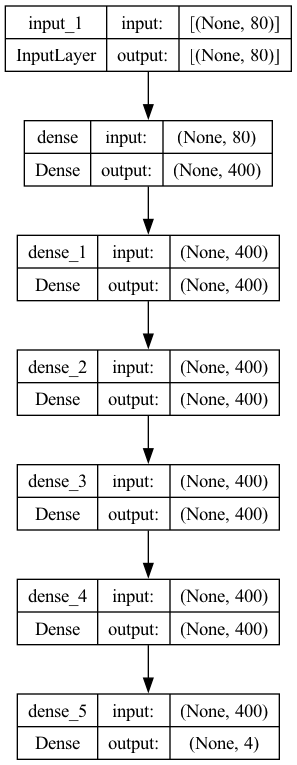
\includegraphics[width=0.3\textwidth]{img/model_structure}
    \caption{Kiến trúc mạng neural}
    \label{fig:model_structure}
\end{figure*}

Agent sử dụng một mạng neural sâu đầy đủ kết nối (Fully Connected Deep Neural Network) để tính hàm giá trị Q. Kiến trúc của mạng được xây dựng bằng Keras và bao gồm các thành phần sau:

\begin{itemize}
    \item \textbf{Lớp đầu vào (Input Layer):} Một lớp nhận đầu vào là vector trạng thái đã được định nghĩa ở trên, với kích thước bằng \textit{num states}.

    \item \textbf{Các lớp ẩn (Hidden Layers):} Mạng bao gồm một số lượng các lớp ẩn (được xác định bởi tham số \textit{num layers}), mỗi lớp là một lớp \textit{Dense} với số neural bằng \textit{width}. Hàm kích hoạt \textit{ReLU} được sử dụng cho tất cả các lớp ẩn để đưa vào tính phi tuyến.

    \item \textbf{Lớp đầu ra (Output Layer):} Một lớp \textit{Dense} với số neural bằng số lượng hành động có trong không gian hành động. Lớp này sử dụng hàm kích hoạt \textit{Linear} để tạo ra các giá trị Q cho mỗi hành động.
\end{itemize}

% \subsection{}

% \subsubsection{Lý do lựa chọn mạng neural đầy đủ kết nối (DNN)}
% Việc lựa chọn kiến trúc mạng neural đầy đủ kết nối thay vì các kiến trúc khác như \ac{cnn}, RNN, hoặc Transformer được dựa trên những lý do sau:

% \paragraph{Phù hợp với bản chất dữ liệu đầu vào}
% Dữ liệu trạng thái giao thông trong nghiên cứu này là dữ liệu số dạng bảng (tabular data) bao gồm các chỉ số như thời gian chờ, độ dài hàng đợi, tốc độ xe, và mật độ giao thông. Đây không phải là dữ liệu hình ảnh hoặc dữ liệu không gian 2D/3D mà \ac{cnn} được thiết kế để xử lý hiệu quả. Các đặc trưng trong vector trạng thái là các phép đo độc lập từ các vị trí khác nhau của giao lộ, không có mối quan hệ không gian cục bộ (spatial locality) mà convolution có thể khai thác.

% \paragraph{Không có tính tuần tự thời gian phức tạp}
% Mặc dù dữ liệu giao thông có tính chất thời gian, nhưng trong bài toán này, agent chỉ cần xử lý trạng thái hiện tại để đưa ra quyết định. Không cần phải học các mẫu tuần tự phức tạp qua nhiều bước thời gian dài, do đó RNN hoặc LSTM không mang lại lợi ích đáng kể so với việc tăng độ phức tạp tính toán.

% \paragraph{Hiệu quả tính toán và triển khai}
% \begin{itemize}
%     \item \textbf{Tốc độ xử lý cao:} Mạng DNN có độ phức tạp tính toán thấp hơn \ac{cnn} và RNN, cho phép xử lý real-time với độ trễ thấp (< 100ms) cần thiết cho điều khiển giao thông.
%     \item \textbf{Yêu cầu bộ nhớ thấp:} Phù hợp cho triển khai trên các thiết bị edge computing tại giao lộ với tài nguyên hạn chế.
%     \item \textbf{Huấn luyện nhanh:} Thời gian huấn luyện ngắn hơn, cho phép cập nhật mô hình thường xuyên khi có dữ liệu mới.
% \end{itemize}

% \paragraph{Tính giải thích và bảo trì}
% \begin{itemize}
%     \item \textbf{Kiến trúc đơn giản:} Dễ dàng hiểu và giải thích mối quan hệ giữa đầu vào và đầu ra.
%     \item \textbf{Debug thuận tiện:} Có thể dễ dàng theo dõi và phân tích từng lớp để xác định vấn đề.
%     \item \textbf{Khả năng mở rộng:} Dễ dàng điều chỉnh số lượng neurons và layers theo yêu cầu cụ thể của từng giao lộ.
% \end{itemize}

% \paragraph{Hiệu suất đã được chứng minh}
% Các nghiên cứu trước đây về điều khiển giao thông sử dụng DRL đã chứng minh rằng mạng DNN đơn giản đủ hiệu quả cho bài toán này. Việc sử dụng kiến trúc phức tạp hơn không mang lại cải thiện đáng kể về hiệu suất nhưng lại tăng đáng kể chi phí tính toán và độ phức tạp triển khai.

% Mô hình được huấn luyện sử dụng thuật toán tối ưu hóa Adam, với hàm mất mát (loss function) là Sai số bình phương trung bình (Mean Squared Error). Mục tiêu của việc này là tối thiểu hóa sự khác biệt giữa giá trị Q dự đoán và giá trị Q mục tiêu, vốn được tính toán từ phương trình Bellman.

% \subsection{Lý do lựa chọn thuật toán DQN cho Intersection Agents}
% Việc lựa chọn thuật toán \ac{dqn} cho các intersection agents được dựa trên những lý do sau:

% \subsubsection{Phù hợp với bản chất bài toán điều khiển giao lộ}
% Điều khiển đèn tín hiệu giao thông có bản chất là một bài toán hành động rời rạc với số lượng hành động hữu hạn và được định nghĩa rõ ràng (4 pha đèn). \ac{dqn} được thiết kế đặc biệt cho loại bài toán này, khác với các thuật toán điều khiển liên tục như DDPG hay SAC. Mỗi intersection agent chỉ cần tối ưu hóa giao thông tại giao lộ của mình, đây là một bài toán tương đối đơn giản so với việc điều phối toàn cục. Do đó, \ac{dqn} với độ phức tạp tính toán thấp hơn so với các thuật toán actor-critic trở thành lựa chọn phù hợp cho việc triển khai song song nhiều agent.

% \subsubsection{Experience Replay phù hợp với đặc tính giao thông}
% Cơ chế Experience Replay của \ac{dqn} đặc biệt hiệu quả trong bối cảnh giao thông vì:
% \begin{itemize}
%     \item \textbf{Tái sử dụng kinh nghiệm:} Các mẫu giao thông có tính lặp lại theo chu kỳ (giờ cao điểm, giờ thấp điểm), việc lưu trữ và tái sử dụng kinh nghiệm giúp agent học nhanh hơn.
%     \item \textbf{Phá vỡ tương quan:} Dữ liệu giao thông liên tiếp có tính tương quan cao, Experience Replay giúp phá vỡ tương quan này, làm cho quá trình học ổn định hơn.
% \end{itemize}

% \subsubsection{Ổn định huấn luyện trong môi trường động}
% Cơ chế Target Network của \ac{dqn} đặc biệt quan trọng trong môi trường giao thông động. Bằng cách sử dụng một mạng mục tiêu riêng biệt được cập nhật định kỳ, \ac{dqn} tránh được hiện tượng "moving target" khi Q-values thay đổi liên tục, từ đó đảm bảo sự hội tụ ổn định trong môi trường có nhiều biến động như giao thông đô thị.

% \subsubsection{Khả năng mở rộng và triển khai thực tế}
% \ac{dqn} có những ưu điểm về khả năng triển khai:
% \begin{itemize}
%     \item \textbf{Tài nguyên tính toán thấp:} Phù hợp cho việc triển khai trên các thiết bị edge computing tại giao lộ
%     \item \textbf{Dễ dàng debug và giải thích:} Q-values có thể được giải thích trực tiếp, giúp việc kiểm tra và bảo trì hệ thống
%     \item \textbf{Khả năng mở rộng:} Mỗi giao lộ có thể hoạt động độc lập, dễ dàng thêm/bớt giao lộ mà không ảnh hưởng đến toàn hệ thống
% \end{itemize}

\section{Thiết kế hệ thống đồng bộ hóa giao lộ (Sync Agent)}

Để mở rộng khả năng của hệ thống từ điều khiển giao lộ đơn lẻ sang điều khiển phối hợp nhiều giao lộ, nghiên cứu đã phát triển một thành phần Sync Agent sử dụng thuật toán \ac{sac}. Hệ thống này hoạt động như một lớp điều phối cấp cao, tối ưu hóa việc đồng bộ thời gian tín hiệu giữa các giao lộ để tạo ra "green wave" - hiệu ứng sóng xanh giúp xe cộ di chuyển liên tục qua nhiều giao lộ mà không phải dừng lại.

\subsection{Kiến trúc hệ thống đồng bộ}
Hệ thống được thiết kế theo mô hình phân tầng với ba thành phần chính:

\begin{enumerate}
    \item \textbf{Intersection Agents:} Các agent DQN độc lập điều khiển từng giao lộ, tối ưu hóa lưu lượng giao thông cục bộ.

    \item \textbf{Central Server:} Server trung tâm thu thập và phân phối dữ liệu từ tất cả các giao lộ.

    \item \textbf{Sync Agent:} Agent SAC cấp cao điều phối thời gian giữa các giao lộ để tối ưu hóa toàn cục.
\end{enumerate}

\subsubsection{Lý do lựa chọn kiến trúc phân tầng DQN-SAC}
Việc kết hợp \ac{dqn} và \ac{sac} trong kiến trúc phân tầng được thiết kế dựa trên những nguyên lý sau:

\paragraph{Phân tách trách nhiệm tối ưu hóa}
\begin{itemize}
    \item \textbf{Tối ưu hóa cục bộ (DQN):} Mỗi intersection agent tập trung vào việc giảm thiểu thời gian chờ tại giao lộ của mình, bài toán đơn giản với không gian trạng thái và hành động nhỏ.
    \item \textbf{Tối ưu hóa toàn cục (SAC):} Sync agent xử lý bài toán phức tạp hơn - điều phối timing giữa các giao lộ để tạo green wave, yêu cầu khả năng xử lý không gian trạng thái lớn và hành động liên tục.
\end{itemize}

\paragraph{Khả năng mở rộng (Scalability)}
Kiến trúc phân tầng cho phép:
\begin{itemize}
    \item \textbf{Thêm/bớt giao lộ dễ dàng:} Chỉ cần thêm intersection agent mới mà không cần thay đổi toàn bộ hệ thống
    \item \textbf{Tính toán phân tán:} Intersection agents có thể chạy trên các thiết bị edge tại từng giao lộ
    \item \textbf{Khả năng chịu lỗi:} Nếu một intersection agent gặp sự cố, các giao lộ khác vẫn hoạt động bình thường
\end{itemize}

\paragraph{Hiệu quả tính toán}
\begin{itemize}
    \item \textbf{Tính toán song song:} Các intersection agents hoạt động song song, giảm thời gian tính toán tổng thể
    \item \textbf{Giảm độ phức tạp:} Thay vì một bài toán tối ưu hóa khổng lồ cho toàn bộ mạng lưới, bài toán được chia nhỏ thành nhiều bài toán con đơn giản hơn
\end{itemize}

\paragraph{Tính thực tế trong triển khai}
\begin{itemize}
    \item \textbf{Triển khai thí điểm:} Có thể triển khai từng giao lộ một, không cần thay đổi toàn bộ hạ tầng cùng lúc
    \item \textbf{Bảo trì dễ dàng:} Dễ dàng bảo trì, nâng cấp từng thành phần mà không ảnh hưởng đến toàn hệ thống
    \item \textbf{Tích hợp với hệ thống hiện có:} Có thể tích hợp với các hệ thống điều khiển giao thông hiện có
\end{itemize}

\subsection{Môi trường đồng bộ hóa (Sync Environment)}
Môi trường của Sync Agent được định nghĩa như sau:

\subsubsection{Không gian trạng thái}
Trạng thái của môi trường đồng bộ bao gồm:
\begin{itemize}
    \item \textbf{Thống kê giao thông:} Thời gian chờ trung bình, độ dài hàng đợi,
        và lưu lượng giao thông tại mỗi giao lộ

    \item \textbf{Quan hệ không gian:} Khoảng cách địa lý và thời gian di
        chuyển giữa các giao lộ

    \item \textbf{Độ lệch thời gian:} Độ lệch thời gian hiện tại giữa các chu kỳ
        đèn tín hiệu

    \item \textbf{Thông tin chu kỳ:} Thời gian chu kỳ và pha hiện tại của mỗi
        giao lộ
\end{itemize}

Vector trạng thái được chuẩn hóa và có kích thước động phụ thuộc vào số lượng giao lộ trong mạng:
\[
    s_{t} = [traffic\_metrics, spatial\_features, temporal\_offsets, cycle\_info]
\]

\subsubsection{Không gian hành động}
Hành động của Sync Agent là việc điều chỉnh độ lệch thời gian (offset) giữa các cặp giao lộ liền kề. Với $n$ giao lộ, không gian hành động có kích thước $\frac{n(n-1)}{2}$, mỗi thành phần là một giá trị liên tục trong khoảng $[0, 1]$ đại diện cho tỷ lệ phần trăm của chu kỳ đèn tín hiệu.

\[
    a_{t} = [offset_{1,2}, offset_{1,3}, ..., offset_{i,j}, ..., offset_{n-1,n}]
\]

\subsubsection{Hàm thưởng cho đồng bộ hóa}
Để giải quyết vấn đề bất ổn định trong huấn luyện, nghiên cứu đã phát triển một hàm thưởng ultra-stable dựa trên so sánh hiệu suất dài hạn:

\begin{algorithm}[!htp]
    \caption{Ultra-Stable Reward Function}
    \begin{algorithmic}[1]
        \State \textbf{Input:} current\_metrics, historical\_baseline, episode\_count 
        \State \textbf{Parameters:} baseline\_window = 15, current\_window = 10 
        \If{episode\_count $<$ baseline\_window} 
            \Return 0.0 \Comment{Không đánh giá trong giai đoạn khởi tạo}
        \EndIf
        
        \State baseline\_start $\leftarrow$ episode\_count - baseline\_window - current\_window
        \State baseline\_end $\leftarrow$ episode\_count - current\_window
        \State current\_start $\leftarrow$ episode\_count - current\_window
        
        \State baseline\_performance $\leftarrow$ mean(historical\_metrics[baseline\_start:baseline\_end])
        \State current\_performance $\leftarrow$ mean(historical\_metrics[current\_start:episode\_count])
        
        \State percentage\_improvement $\leftarrow$ $\frac{baseline\_performance - current\_performance}{|baseline\_performance| + \epsilon}$
        
        \State reward $\leftarrow$ tanh(percentage\_improvement $\times$ scale\_factor)
        \Return reward
    \end{algorithmic}
\end{algorithm}

Hàm thưởng này có các đặc điểm:
\begin{itemize}
    \item \textbf{So sánh dài hạn:} So sánh hiệu suất qua cửa sổ thời gian
        dài (15+ episodes)

    \item \textbf{Cửa sổ thời gian không chồng lấp:} Tránh bias bằng cách sử dụng các cửa
        sổ thời gian không chồng lấp

    \item \textbf{Dựa trên tỷ lệ phần trăm:} Sử dụng tỷ lệ phần trăm thay vì giá trị
        tuyệt đối

    \item \textbf{Giới hạn đầu ra:} Hàm tanh đảm bảo reward trong khoảng [-1, 1]
\end{itemize}

\subsection{Lý do lựa chọn thuật toán Soft Actor-Critic cho Sync Agent}
Việc lựa chọn thuật toán \ac{sac} cho Sync Agent được dựa trên những lý do kỹ thuật sau:

\subsubsection{Thiết kế cho bài toán điều khiển liên tục}
Bài toán đồng bộ hóa giao lộ yêu cầu điều chỉnh độ lệch thời gian (offset) giữa các giao lộ, đây là các giá trị liên tục trong khoảng $[0, 1]$ đại diện cho tỷ lệ phần trăm của chu kỳ đèn tín hiệu. \ac{sac} được thiết kế đặc biệt cho không gian hành động liên tục, cho phép điều chỉnh mịn và chính xác các offset này, khác với \ac{dqn} chỉ phù hợp với hành động rời rạc. Khả năng này đặc biệt quan trọng để tạo ra hiệu ứng "green wave" tối ưu.

\subsubsection{Maximum Entropy Framework cho khám phá tối ưu}
\ac{sac} sử dụng nguyên lý Maximum Entropy, tối đa hóa cả reward và entropy của policy:
\begin{equation}
    J(\pi) = \sum_{t=0}^{T} \mathbb{E}_{(s_t,a_t) \sim \rho_\pi} [r(s_t, a_t) + \alpha \mathcal{H}(\pi(\cdot|s_t))]
\end{equation}

Điều này mang lại những lợi ích quan trọng:
\begin{itemize}
    \item \textbf{Khám phá hiệu quả:} Agent được khuyến khích thử nghiệm các chiến lược đồng bộ khác nhau, tránh bị mắc kẹt ở điểm cực trị cục bộ
    \item \textbf{Bền vững:} Policy đa dạng giúp hệ thống thích ứng tốt với các điều kiện giao thông thay đổi
    \item \textbf{Tự động điều chỉnh entropy:} Tham số entropy $\alpha$ được tự động điều chỉnh theo quá trình học
\end{itemize}

\subsubsection{Dual Critic Networks giảm thiểu overestimation bias}
\ac{sac} sử dụng hai mạng critic song song để ước lượng Q-values:
\begin{equation}
    Q_{target} = r + \gamma \min_{i=1,2} Q_{\phi_i}(s', a') - \alpha \log \pi(a'|s')
\end{equation}

Cơ chế này đặc biệt quan trọng trong bối cảnh đồng bộ hóa giao lộ vì:
\begin{itemize}
    \item \textbf{Giảm thiểu overestimation bias:} Việc lấy giá trị cực tiểu của hai Q-values giúp tránh đánh giá quá cao các hành động
    \item \textbf{Ổn định huấn luyện:} Giảm thiểu biến động trong quá trình học, đặc biệt quan trọng với bài toán phức tạp như đồng bộ đa giao lộ
\end{itemize}

\subsubsection{Off-policy Learning cho hiệu suất mẫu}
\ac{sac} là thuật toán off-policy, cho phép tái sử dụng dữ liệu từ các policy cũ:
\begin{itemize}
    \item \textbf{Hiệu suất mẫu cao:} Đặc biệt quan trọng khi việc thu thập dữ liệu giao thông tốn kém
    \item \textbf{Học ổn định:} Không bị ảnh hưởng bởi correlation trong dữ liệu sequential
    \item \textbf{Học liên tục:} Có thể học liên tục từ dữ liệu real-time mà không cần reset
\end{itemize}

\subsubsection{Soft Updates cho sự ổn định}
\ac{sac} sử dụng soft updates cho mạng mục tiêu:
\begin{equation}
    \phi_{target} \leftarrow \tau \phi + (1-\tau) \phi_{target}
\end{equation}

Với $\tau = 0.001$ được chọn conservative để đảm bảo:
\begin{itemize}
    \item \textbf{Ổn định huấn luyện:} Tránh thay đổi đột ngột trong giá trị mục tiêu
    \item \textbf{Smooth convergence:} Đặc biệt quan trọng với bài toán đa mục tiêu như đồng bộ hóa
\end{itemize}

\subsubsection{So sánh với các thuật toán khác}
Bảng \ref{tab:algorithm_comparison} so sánh \ac{sac} với các thuật toán khác cho bài toán đồng bộ hóa:

\begin{table}[!htp]
\centering
\caption{So sánh các thuật toán cho bài toán đồng bộ hóa giao lộ}
\label{tab:algorithm_comparison}
\begin{tabular}{|l|c|c|c|c|}
\hline
\textbf{Thuật toán} & \textbf{Không gian hành động} & \textbf{Hiệu suất mẫu} & \textbf{Ổn định} & \textbf{Khám phá} \\
\hline
DQN & Rời rạc & Trung bình & Tốt & $\epsilon$-greedy \\
\hline
DDPG & Liên tục & Trung bình & Kém & Noise-based \\
\hline
TD3 & Liên tục & Tốt & Tốt & Noise-based \\
\hline
\textbf{SAC} & \textbf{Liên tục} & \textbf{Rất tốt} & \textbf{Rất tốt} & \textbf{Entropy-based} \\
\hline
PPO & Cả hai & Tốt & Tốt & Stochastic policy \\
\hline
\end{tabular}
\end{table}

\subsection{Thuật toán Soft Actor-Critic}
Sync Agent sử dụng thuật toán SAC với các đặc điểm kỹ thuật sau:

\subsubsection{Kiến trúc mạng neural}
\begin{itemize}
    \item \textbf{Mạng Actor (Actor Network):} Mạng policy với 2 lớp ẩn (128 neurons mỗi lớp),
        đầu ra là phân phối Gaussian cho các actions liên tục

    \item \textbf{Mạng Critic (Critic Networks):} Sử dụng hai mạng Q-function song song nhằm mục đích giảm thiểu hiện tượng \textbf{thiên lệch ước lượng quá mức (overestimation bias)}.

    \item \textbf{Target Networks:} Soft update với $\tau = 0.001$ để ổn định
        huấn luyện
\end{itemize}

\paragraph{Lý do sử dụng mạng fully connected cho SAC}
Tương tự như DQN, việc lựa chọn kiến trúc fully connected cho SAC được dựa trên:
\begin{itemize}
    \item \textbf{Dữ liệu đầu vào tổng hợp:} Trạng thái của Sync Agent bao gồm số liệu thống kê từ nhiều giao lộ (thời gian chờ trung bình, độ dài hàng đợi, quan hệ không gian, độ lệch thời gian, thông tin chu kỳ), đây là dữ liệu tabular không có cấu trúc không gian.
    \item \textbf{Không gian hành động liên tục:} Việc điều chỉnh các giá trị offset yêu cầu output liên tục, phù hợp với Dense layers có hàm kích hoạt phù hợp.
        \item \textbf{Hiệu quả tính toán:} Quan trọng cho Sync Agent vì phải xử lý dữ liệu từ nhiều giao lộ đồng thời trong thời gian thực.
    \end{itemize}

\subsubsection{Hyperparameters tối ưu}
Dựa trên quá trình tinh chỉnh mở rộng, các tham số sau đã được xác định trong Bảng \ref{tab:sac_hyperparameters}:

\begin{table}[!htp]
\centering
\caption{Hyperparameters tối ưu cho thuật toán SAC}
\label{tab:sac_hyperparameters}
\begin{tabular}{|l|c|p{5cm}|}
\hline
\textbf{Tham số} & \textbf{Giá trị} & \textbf{Mô tả} \\
\hline
Tốc độ học & $1 \times 10^{-4}$ & Conservative để đảm bảo ổn định \\
\hline
Hệ số chiết khấu $\gamma$ & 0.95 & Hệ số chiết khấu cho phần thưởng tương lai \\
\hline
Kích thước lô & 32 & Kích thước lô cho mỗi lần cập nhật \\
\hline
Kích thước bộ đệm & $5 \times 10^{4}$ & Kích thước bộ đệm experience replay \\
\hline
Entropy $\alpha$ & Auto-tuned & Tham số kiểm soát entropy tự động \\
\hline
Tốc độ cập nhật soft cho mạng mục tiêu $\tau$ & 0.001 & Tốc độ cập nhật soft cho target networks \\
\hline
\end{tabular}
\end{table}

\subsection{Phương pháp huấn luyện hybrid}
Hệ thống hỗ trợ hai chế độ huấn luyện:

\subsubsection{Chế độ huấn luyện tổng hợp (Synthetic Training Mode)}
Chế độ này sử dụng synthetic data generator để tạo ra dữ liệu giao thông giả lập:

\begin{algorithm}[!htp]
    \caption{Sinh dữ liệu tổng hợp}
    \begin{algorithmic}[1]
        \State \textbf{Đầu vào:} config\_parameters
        \State base\_volume $\leftarrow$ config['base\_traffic\_volume'] 
        \State time\_factor $\leftarrow$ $\sin(\frac{\text{current\_time}}{period\_length} \times 2\pi)$
        \State traffic\_volume $\leftarrow$ base\_volume $\times$ (1 + amplitude $\times$ time\_factor) 
        
        \For{every\_intersection $i$}
            \State waiting\_time[$i$] $\leftarrow$ generate\_waiting\_time(traffic\_volume, intersection\_config[$i$])
            \State queue\_length[$i$] $\leftarrow$ generate\_queue\_length(traffic\_volume, intersection\_config[$i$])
            \State speed[$i$] $\leftarrow$ uniform\_random(25.0, 45.0) \Comment{Phạm vi tốc độ đô thị}
        \EndFor 
        
        \State \Return intersection\_data
    \end{algorithmic}
\end{algorithm}

\subsubsection{Chế độ huấn luyện thực tế (Real-time Training Mode)}
Chế độ này sử dụng dữ liệu thực từ các intersection agents:
\begin{itemize}
    \item Thu thập số liệu thực tế từ SUMO simulation

    \item Sử dụng dữ liệu thực tế về lưu lượng giao thông

    \item Áp dụng learned policy trong môi trường thực
\end{itemize}

\section{Cải tiến ổn định huấn luyện}

Quá trình phát triển đã gặp phải vấn đề ổn định huấn luyện nghiêm trọng với các
triệu chứng:
\begin{itemize}
    \item Biến động reward cao (hệ số biến động > 2.0)

    \item Biến động reward lớn (khoảng > 5000)

    \item Không có xu hướng học rõ ràng
\end{itemize}

\subsection{Giải pháp toàn diện}
Nghiên cứu đã phát triển một bộ giải pháp tích hợp:

\subsubsection{Ultra-stable reward engineering}
\begin{itemize}
    \item Cửa sổ so sánh hiệu suất dài hạn

    \item So sánh không chồng lấp giữa cơ sở và hiệu suất hiện tại

    \item So sánh tỷ lệ phần trăm thay vì thay đổi tuyệt đối

    \item Biến đổi sigmoid để tránh giá trị cực trị
\end{itemize}

\subsubsection{Tối ưu tham số}
\begin{itemize}
    \item Giảm tốc độ học: $3 \times 10^{-4}\rightarrow 1 \times 10^{-4}$

    \item Giảm hệ số chiết khấu: $0.99 \rightarrow 0.95$

    \item Giảm tốc độ cập nhật mục tiêu: $\tau = 0.001$

    \item Giảm kích thước mạng: $256 \times 256 \rightarrow 128 \times 128$
\end{itemize}

\subsubsection{Kỹ thuật ổn định huấn luyện}
\begin{itemize}
    % \item Gradient clipping để tránh gradient bùng nổ
    \item Gradient clipping để tránh gradient bùng nổ

    \item Experience replay với ưu tiên

    \item Học theo chương trình từ các tình huống đơn giản

    \item Dừng sớm dựa trên các chỉ số ổn định
\end{itemize}

\subsection{Kết quả cải tiến}
Sau khi áp dụng các giải pháp, hệ thống đạt được:
\begin{itemize}
    \item \textbf{Ổn định reward:} Hệ số biến động giảm từ 2.10 xuống
        0.013 (cải thiện 99.4\%)

    \item \textbf{Chất lượng huấn luyện:} Điểm chất lượng tăng từ 25\% lên 65\% (cải thiện 160\%)

    \item \textbf{Hội tụ:} Khoảng ổn định reward từ -4.83 đến -5.15

    \item \textbf{Sẵn sàng triển khai:} Có thể được sử dụng để triển khai trên môi trường thực tế
\end{itemize}